\documentclass[12pt]{article}
\usepackage{amsmath}
\usepackage{amssymb}
%\usepackage{hyperref}
\usepackage{epsfig,graphicx,amsmath}
\usepackage{amsfonts}
\usepackage{enumerate}
\usepackage{amsfonts}
\usepackage{amssymb}
\usepackage{amsthm}


\newcommand{\mb}[1]{\mbox{\boldmath$#1$}}
\newcommand{\p}{\partial}
\newcommand{\ds}{\displaystyle}
\newcommand{\beq}{\begin{eqnarray}}
\newcommand{\beqq}{\begin{eqnarray*}}
\newcommand{\eeq}{\end{eqnarray}}
\newcommand{\eeqq}{\end{eqnarray*}}
\newcommand{\eps}{\varepsilon}
\newcommand{\erf}{\mbox{erf}}
\newcommand{\erfi}{\mbox{erfi}}
\newcommand{\Ei}{\mbox{Ei}}
\newcommand{\x}{\mbox{\boldmath$x$}}
\newcommand{\Aa}{\mbox{\boldmath$A$}}
\newcommand{\rr}{\mbox{\boldmath$r$}}
\newcommand{\As}{\mbox{\boldmath$a$}}
\newcommand{\y}{\mbox{\boldmath$y$}}
\newcommand{\z}{\mbox{\boldmath$z$}}
\newcommand{\J}{\mbox{\boldmath$J$}}
\newcommand{\ET}{\mbox{\boldmath$\eta$}}
\newcommand{\n}{\mbox{\boldmath$n$}}
\newcommand{\X}{\mbox{\boldmath$X$}}
\newcommand{\Y}{\mbox{\boldmath$Y$}}
\newcommand{\Yy}{\mbox{\boldmath$y$}}
\newcommand{\Z}{\mbox{\boldmath$Z$}}
\newcommand{\w}{\mbox{\boldmath$w$}}
\newcommand{\vv}{\mbox{\boldmath$v$}}
\newcommand{\bb}{\mbox{\boldmath$b$}}
\newcommand{\Bb}{\mbox{\boldmath$b$}}
\newcommand{\B}{\mbox{\boldmath$B$}}
\newcommand{\ALPHA}{\mbox{\boldmath$\alpha$}}
\newcommand{\aaa}{\mbox{\boldmath$a$}}
\newcommand{\C}{\mbox{\boldmath$C$}}
\newcommand{\SSigma}{\mbox{\boldmath$\Sigma$}}
\newcommand{\mmu}{\mbox{\boldmath$\mu$}}
\newcommand{\IIm}{\mbox{\boldmath$I_m$}}
\newcommand{\mean}[1]{\langle #1\rangle}
\newcommand{\diffunit}{$\mu$m$^2$.s$^{-1}$}
\newcommand{\Li}{\mbox{Li}}
\newcommand{\thet}{\mbox{\boldmath$\theta$}}
\newcommand{\intR}{\int\limits_{\mathbb{R}}}
\newcommand{\intRm}{\int\limits_{\mathbb{R}^m}}
\newcommand\norm[1]{\left\lVert#1\right\rVert}
%\definecolor{red}{rgb}{1,0,0}

\usepackage{color}
\usepackage{float}
\begin{document}	
\title{ Material and methods}
\maketitle

\section{Result section : Modeling Nucleosome reorganization after damages}

To estimate the nucleosome reorganization following DNA damages, we built a model where redistribution can be due either to chromatin de-compaction or nucleosome sliding along the chromatin or both of them.  Because the sliding loss is inaccessible experimentally, we use the model to assess the relative contribution of these two processes to nucleosomes eviction from the region of interest (ROI).

The model (presented in Material and methods) follows the DNA $d(U)$ and nucleosome $h(U)$ fraction of signal loss from ROI and for a given UV does $U$, which are calibrated from the measured  H3.3 signal loss and DNA signal loss respectively (Fig. 3A-D). 


\section{Material and methods: Modeling  histones redistribution following UV damages}
We present here a model for nucleosomes and chromatin re-organization following UV damages. 

\subsection{Dynamics of histones following UV damages in the region of interest}
Following the experimental protocol, the initial damage circular region (IDR) induced by the laser beam is centered around the focal point (origin of the coordinates), with an exposure time $u \in [5-100]$ ms. Following laser induction, because the tagged damage points region increases and reaches it maximal size after 15 minutes, this domain is defined as the region of Interest (ROI), in which both histone and DNA signal is measured 15 minutes post UVC and compared to values before induction (see also the empirical definition in XXX). 

We assume that the loss of DNA and nucleosomes signal is due to two mechanisms: one is nucleosome sliding along the chromatin and outward in the direction of the ROI's boundary, and the second is chromatin expansion or unfolding. First, the nucleosomes involved in sliding are those that contained damaged DNA wrapped around them. In this model, a nucleosome cannot detach from the chromatin or pass through another one. The exact mechanism of motion is not considered here because we will only consider the steady-state final result, defined at 15 minutes post UVC. In the second mechanism, recruitment of repair proteins to the damage region unfolds the chromatin and as a result  both nucleosome and DNA signal is lost in equal proportion (Fig. 3XXX) as is being pushed out of the ROI with the expansion of the DR. Note that due to expansion of chromatin, the DNA and nucleosomes located in the annulus between the ROI and IDR is going to be extruded from the ROI.

In the model, due to the radial symmetry, we consider that chromatin is a single wire of total length $l$, with one end fixed at the origin and the other at the boundary of the $IDR$ of radius $R_0$. There are $N_0$ histones on this chromatin wire.  The ROI region is considered to be a circle of area $A(u)$, with, and $u$ the UV-dose. We set the number of nucleosomes in the DR as $N(u)$.

\subsection{Fraction of DNA and nucleosome loss }\label{subsection:fractionOfDNAandNucleosomeLoss}
We assume an initial uniform distribution of both DNA and nucleosome. 
We shall now compute the fraction of DNA loss (resp. nucleosomes) $D(u)$ (resp. $H(u)$) in the ROI 15 minutes post UVC. By construction, $D(u)$ is given by the ratio of the amount of DNA in the annulus between the ROI and $A_0$ to the total amount in the ROI, while $H(u)$ is the sum of the nucleosomes that have been translocated with the DNA plus the ones that are sliding out, resulting in the following formulas
\begin{eqnarray*}
D(u)&=& \frac{A(u)/A_0 -1}{A(u)/A_0} \\
H(u)&=&D(u)+\frac{N(0)-N(u)}{N(0)A(u)/A_0}.
\end{eqnarray*}
with $I_u$ the area of the initial damage region.
In order to evaluate the functions above, we will now construct models for the functions $A(u)$ and $N(u)$.

\subsection{Deriving the number of damages $T(u)$}
We assume here that the rate of accumulating DNA damages, $T(u)$, in the initial damage region is increasing proportional to the undamaged DNA in the initial damage region, $I_u$.
\begin{equation}
\frac{dT(u)}{du}=k_T\left(T_{max}-T(u)\right)
\end{equation}
with $k_T$ the rate constant, and $T_{max}$ the maximal number of damages possible in $I_u$. 
Using the initial condition $T(0) = 0$ the solution is
\begin{equation}
T(u) = T_{max}\left(1-\exp(-k_T u)\right) 
\end{equation}
Because we cannot have two damages at the same position on the DNA, and the number of damages is bounded from above by $T_{max}$, we can treat the quantity 
\begin{equation*}
T(u)/T_{max}
\end{equation*}
as the fraction of chromatin length damaged, or as the damage coverage percentage. 

\subsection{Deriving the function $A(u)$ and $N(u)$ from the dynamics of loss}
We now turn to construct a model for the number of nucleosomes $N(u)$ left in ROI, as a function of the UV dose, $u$. Although the exact mechanism by which nucleosomes are lost is not known, we assume here that $N(u)$ is proportional to the rate of accumulation of DNA damages $T(u)$ with increasing uv dose. The nucleosome lost by sliding are initially located on a fixed chromatin of length $l$ in the IDR. We assume that additional damages caused by increasing UV dose, distribute uniformly on the  The fraction out of the total chromatin length in the IDR that nucleosomes are occupying is $N(u)b/l$, with $b$ the length of DNA wrapped on a histone. Therefore, with an addition of $dT(u)$ damages, the number of histone-wrapped DNA which has at least one damage is a multiplication of the fraction of the chromatin damaged with the fraction of chromatin length nucleosomes are occupying, i.e. $ \frac{N(u)bdT}{lT_{max}} $. Therefore, the equation for the number of nucleosomes left in the ROI 15 post UVC as a function of the uv dose can be written as
\begin{equation*}
\frac{dN(u)}{du} = -k_NN(u)\frac{dT(u)}{du}
\end{equation*}
with $k_N$ a constant describing the rate of histone depletion from the ROI due to sliding. Using the initial condition $N(0) = N_0$, the solution is given by
\begin{equation}\label{eq:NumHistones}
N(u) = N_0\exp\left(-k_N\left(1-\exp(-k_Tu)\right)\right).
\end{equation}
Note that $N(u)$ represents the number of nucleosomes left in the ROI 15 minutes post UVC for a given UV dose $u$.

To compute the dynamics of $A(u)$, we assume that with each damage position on the DNA there are repair protein attached to it which occupy space and collectively increase the area of the IDR. Damaged positions on the DNA, which are wrapped on histones needs to be exposed. With their exposure, repair proteins attach to the damage point. Because the length of the chromatin in the damage region does not change with expansion, only the portion of the chromatin occupied with nucleosomes change with UV dose (at saturation). Therefore, if $l$ is the chromatin length in the IDR, and $b$ is the length of chromatin wrapped around a single histone, then the portion of the chromatin occupied by histones at saturation is $N(u)b/l$. For each UV dose, every point in a concentric ring around the laser's focal point is equally probable to be damaged. The opening is then related to the additional exposure of damages point which were wrapped on histones. 

\begin{equation}\label{dralpha}
\frac{dA(u)}{du}=-k_A\frac{dN(u)}{du}+k_B\frac{dT(u)}{du}
\end{equation}
where $k_A$ is a constant. Using the initial condition $A(0)=A_0$, we find 
\begin{equation}\label{eq:expansionFactor}
A(u) = A_0 +k_AN_0\left(1-\exp\left(-k_NT(u)\right)\right) +k_BT(u)
\end{equation}
with $A_0$ being a theoretical value for measurement in the absence of UV radiation in an area $I_u$. We interpret the increase in ROI radius with the UV dose as follows: while nucleosomes are sliding outside, repair proteins are invading and then binding at sites of DNA damages. The accumulation of these proteins are producing force on the chromatin that result in the radial outward expansion. In our model, the amount of repair proteins is directly proportional to the number of exposed damage points, which is also proportional to the number of nucleosome in the damage region.

We can now use these derivations to compute the fraction of DNA and nucleosome loss. The fraction of histone loss for UV dose $u$ is given by
\begin{equation}\label{eq:histoneLoss}
H(u) = \frac{(A(u)/I_u)-1}{(A(u)/I_u)} +\frac{N_0-N(t)}{N_0(A(u)/I_u)}=1-\frac{(N(t)/N_0)}{(A(u)/I_u)}
\end{equation}
Substituting expressions \ref{eq:NumHistones}-\ref{eq:expansionFactor} into \ref{eq:histoneLoss}, we obtain

\subsection{Contribution of opening to the total DNA signal loss}

The expansion of the damage region post UV is composed of two contributions, one of the sliding of histones and the second from chromatin de-compaction.
The de-compaction by itself contributes to the opening a fraction related to the second term on the right hand side of equation \ref{dralpha}, that is 
\begin{equation}
\frac{dA_{opening}}{du}=+k_B\frac{dT(u)}{du}
\end{equation}
For which the solution is 
\begin{equation}
A(u)_{opening}= A(0)_{opening}+k_BT_{max}(1-\exp(-k_Tu))
\end{equation}


\subsection{Dependency on UV dose and final expression for the nucleosomes $H(u)$ and DNA $D(u)$ loss}

The number of damages $\bar{D}$ increases with the UV dose, but decreases with the distance from the laser's focal point. To obtain an exact expression for $\bar{D}$, we use the UVC intensity $I$ which decays with the distance from the focal point as the inverse-square law of laser intensity: $I \sim \frac{U}{r^2}$, where $r$ is the distance from focal point, and $U$ the UV-exposure time.

For a uniform DNA distribution, the amount enclosed in concentric rings around the focal point increases linearly with $r$. Therefore, the number of damages in a concentric two-dimensional ring of radius $r$ and size $dr$ is ${D}= \frac{rU}{r^2}=\frac{U}{r}dr$. The average of $\bar{D}$ in the entire circular region of radius $R$ is
\begin{equation*}
\bar{D}(R) = C\int_0^R \frac{U}{r} rdr = CUR,
\end{equation*}
where $C$ is constant. We conclude that the average number of damages per unit chromatin length is thus proportional to $U$ and thus the total loss of histones at saturation time $t_{s}$ depends on the UV dose and can be computed from relation \ref{eq:totalHistoneLoss} by
\begin{equation}\label{eq:totalHiostoneLossVsUV}
h(U)=h(t_s)=1-\frac{\exp(-\beta U)}{ 1+C_2(1-\exp(-\beta U))}.
\end{equation}
where $\beta=\frac{Ck_rt_s}{l}$, represent the decay of $h$ with respect to the UV does and $C_2=k_RN_0$ is a constant. Similarly, the DNA loss at time $t_{s}$ is given by
\begin{equation}\label{eq:dStSt}
d(t_s)= 1-\frac{1}{\alpha(t_s)}.
\end{equation}
Using expressions \ref{eq:expansionFactor} and \ref{eq:dStSt}, we obtain
\begin{equation}\label{eq:dnaLoss}
d(U)= \frac{C_2(1-\exp(-\beta U))}{1+C_2(1-\exp(-\beta U))}
\end{equation}
which is UV dose dependent function.


%%%%%%%%%%%%%%%%%%%%%%%%%%%%%%%%%%%%%%%%%%%%%%%%%%%%%%%%%%%
\subsection{Parameter fit for $h$ and DNA $d$ loss}\label{subsection:parameterFit}
%%%%%%%%%%%%%%%%%%%%%%%%%%%%%%%%%%%%%%%%%%%%%%%%%%%%%%%%%%%
We now use eqs. \ref{eq:totalHiostoneLossVsUV} to fit the experimental data describing the fraction of histone loss from the ROI 15 minutes post UVC. Since $d(U)$ and $h(U)$ share similar parameters, only $h(U)$ will be used. A classical fitting procedure, where we excluded the measurement of histone loss at 100 ms UVC dose, we find
\begin{eqnarray*}
\beta &=&  0.007\\
C_2   &=&  0.78
\end{eqnarray*}
where the square error (SSE) is 0.0225 (resp. 0.0173) for $h(U)$ (resp. $d(U)$).
%%%%%%%%%%%%%%%%%%%%%%%%%%%%%%%%%%%%%%%%%%%%%%%%%%%%%%%%%%%
\begin{figure}[http!]
\centering
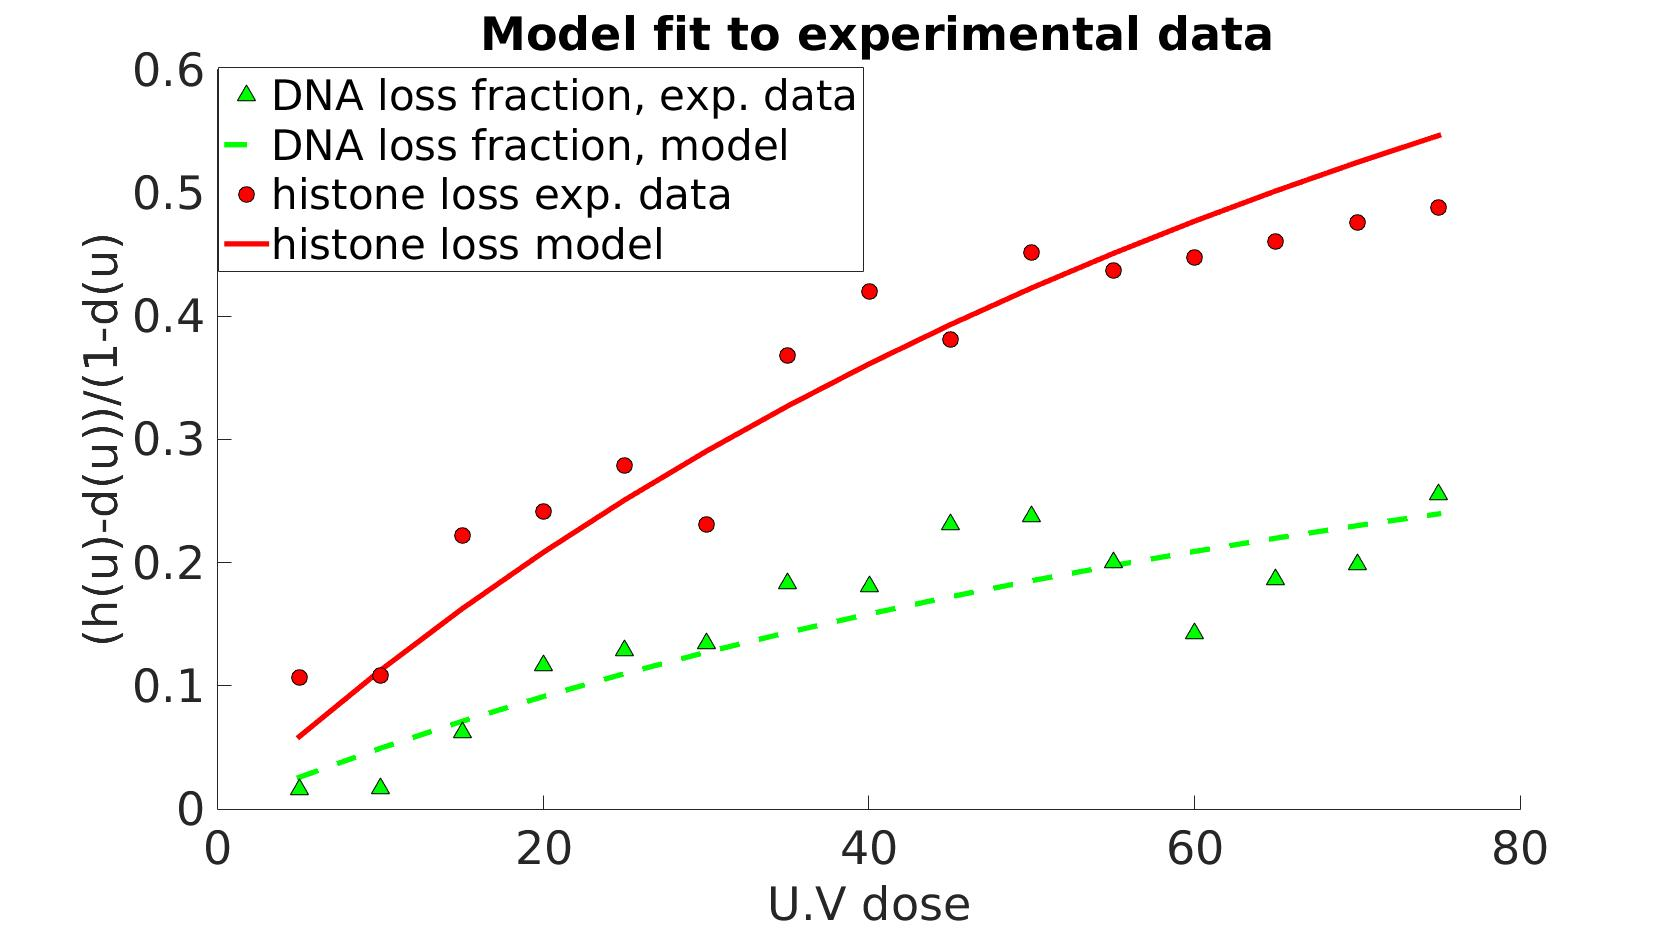
\includegraphics[width=0.5\linewidth, height=0.3\textheight]{histoneAndDnaVsUvDoseModelFit}
\caption{\textbf{Histone loss (red): experimental data (circle) versus analytical curve (continuous)}. The fit is obtained from  eq. \ref{eq:totalHiostoneLossVsUV}.  The parameters are $C_2 =0.78,\quad \beta=0.007$. These parameter are used in eq. \ref{eq:dnaLoss} for DNA loss (green dashed curve) plotted against experimental points (green triangles).}
\label{fig:histoneAndDnaVsUvDoseModelFit}
\end{figure}

%%%%%%%%%%%%%%%%%%%%%%%%%%%%%%%%%%%%%%%%%%%%%%%%%%%%%%%%%%%
\subsection{Fraction of nucleosome loss attributed to sliding}\label{subsection:lossAttributedToSliding}
%%%%%%%%%%%%%%%%%%%%%%%%%%%%%%%%%%%%%%%%%%%%%%%%%%%%%%%%%%%
Using parameters of subsection \ref{subsection:parameterFit}, we can now calculate the fraction of histones loss attributed to sliding $h(U)-d(U)$. The result is show in Figure \ref{fig:hVsUVDoseModelFit01}.
%%%%%%%%%%%%%%%%%%%%%%%%%%%%%%%%%%%%%%%%%%%%%%%%%%%%%%%%%%%
\begin{figure}[http!]
\centering
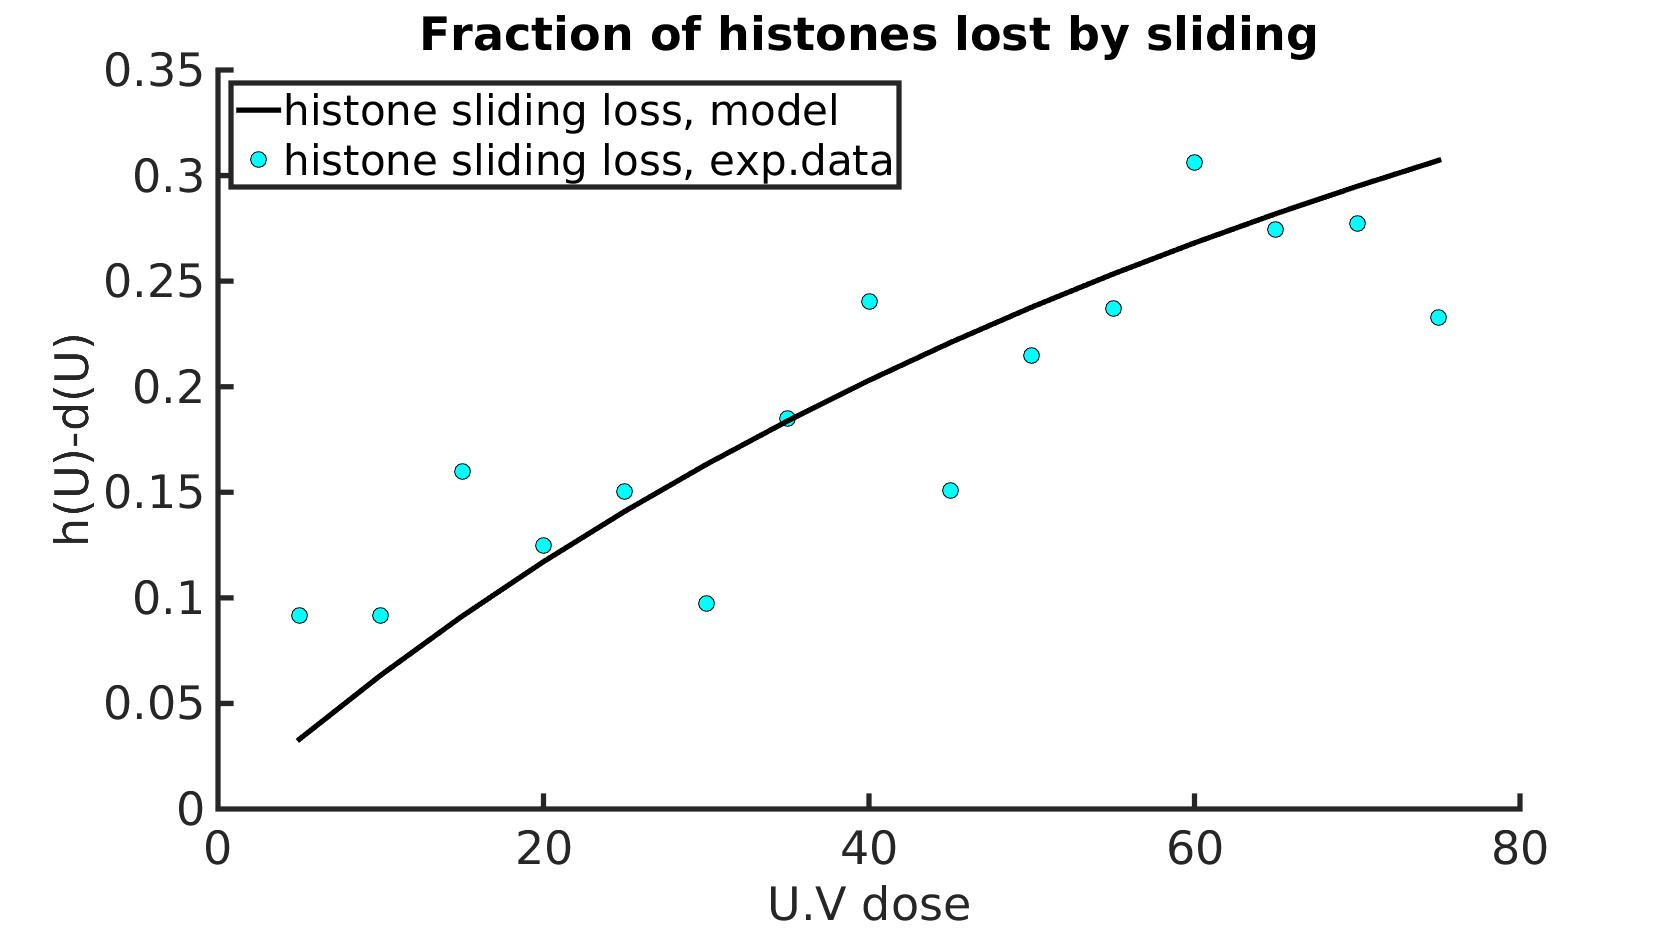
\includegraphics[width=0.5\linewidth, height=0.3\textheight]{hVsUVDoseModelFit}
\caption{\textbf{Fraction $h(U)-d(U)$ of histone loss attributed to sliding} plotted against the experimental data.}
\label{fig:hVsUVDoseModelFit01}
\end{figure}
%%%%%%%%%%%%%%%%%%%%%%%%%%%%%%%%%%%%%%%%%%%%%%%%%%%%%%%%%%%
The fraction of histone sliding out of the DR is $\frac{h(U)-d(U)}{1-d(U)}$. Figure \ref{fig:histoneSlideFromDamageRegionComparision} shows the result of the model and a linear approximation, both capture well the increase in sliding fraction in the UV dose range of the experimental data, with near equal variations from experimental data (SSE model = 0.028, SSE linear fit= 0.039).
%%%%%%%%%%%%%%%%%%%%%%%%%%%%%%%%%%%%%%%%%%%%%%%%%%%%%%%%%%%
\begin{figure}[http!]
	\centering
	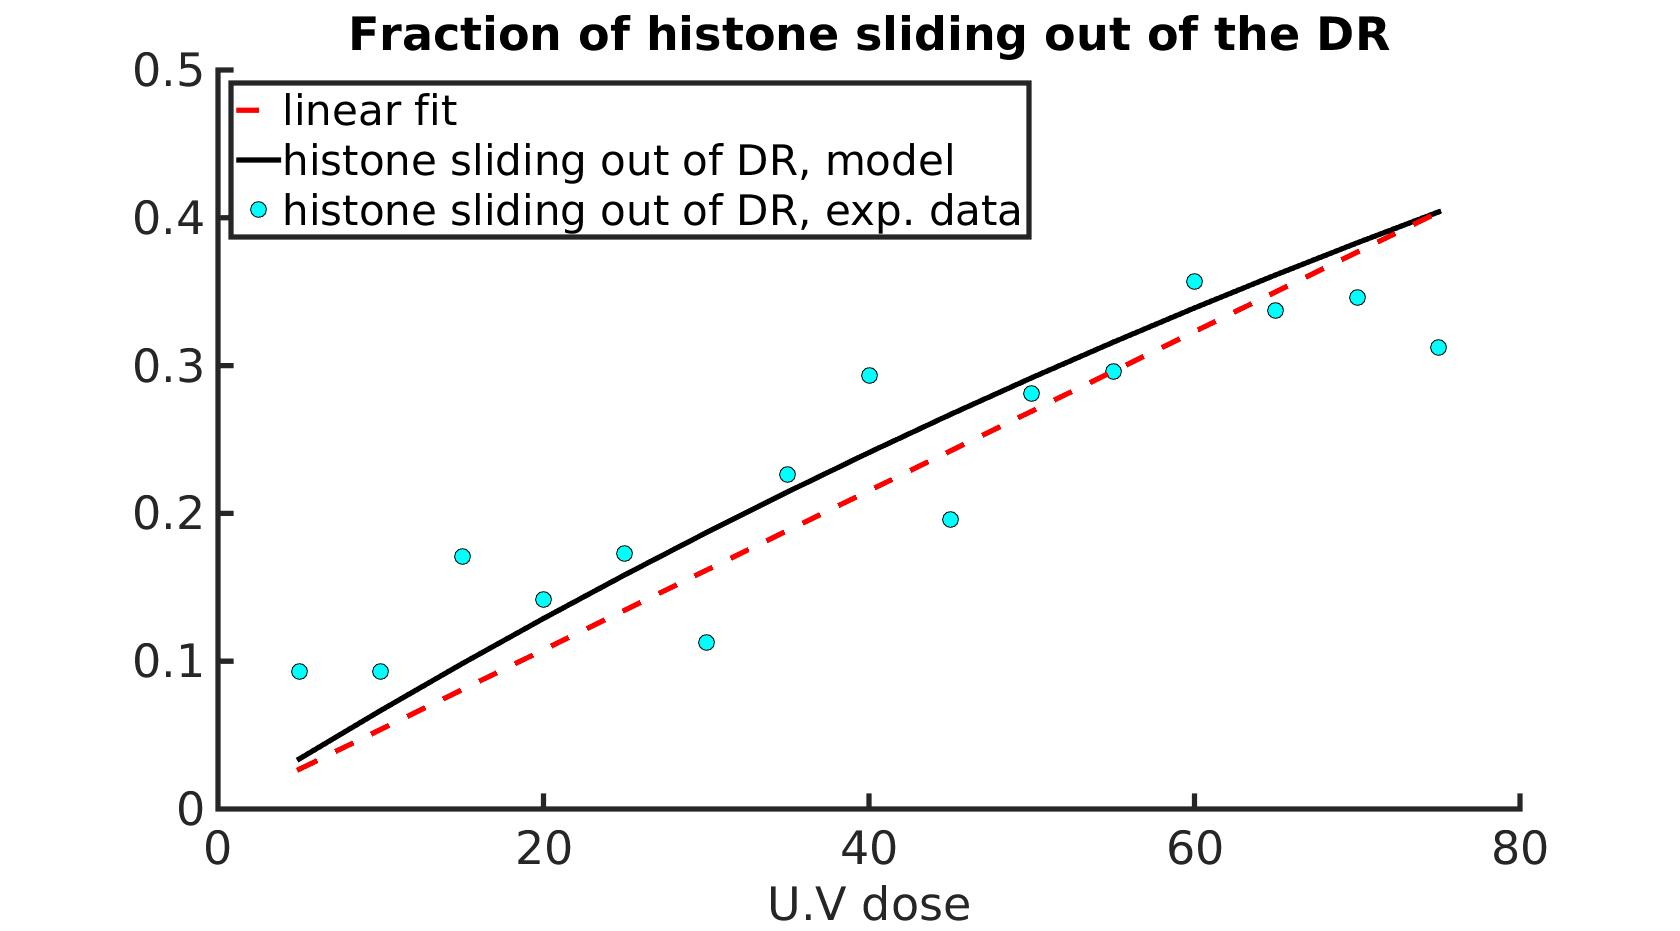
\includegraphics[width=0.7\linewidth, height=0.3\textheight]{histoneSlideFromDamageRegionComparision}
	\caption{\textbf{Fraction of lost histones from the DR due to sliding.} The model (black curve) shows a near linear increase in the range of UV dosage tested for the experimental data $(h(U)-d(U))/(1-d(U))$. A linear fit approximation (dashed red line) shows a similar behavior to the model, although with higher SSE (model =0.028, vs. linear fit=0.039 ) }
	\label{fig:histoneSlideFromDamageRegionComparision}
\end{figure}
%%%%%%%%%%%%%%%%%%%%%%%%%%%%%%%%%%%%%%%%%%%%%%%%%%%%%%%%%%%
Interestingly we find that, independent of the UV dose, the relative contribution of histone sliding to the total histone loss remains a constant of roughly 56\% of the total loss (Figure \ref{fig:relativeSlidingContribution}), and in general is given by $1-C_2/(C_2+1)$.

%%%%%%%%%%%%%%%%%%%%%%%%%%%%%%%%%%%%%%%%%%%%%%%%%%%%%%%%%%%
\begin{figure}[H]
\centering
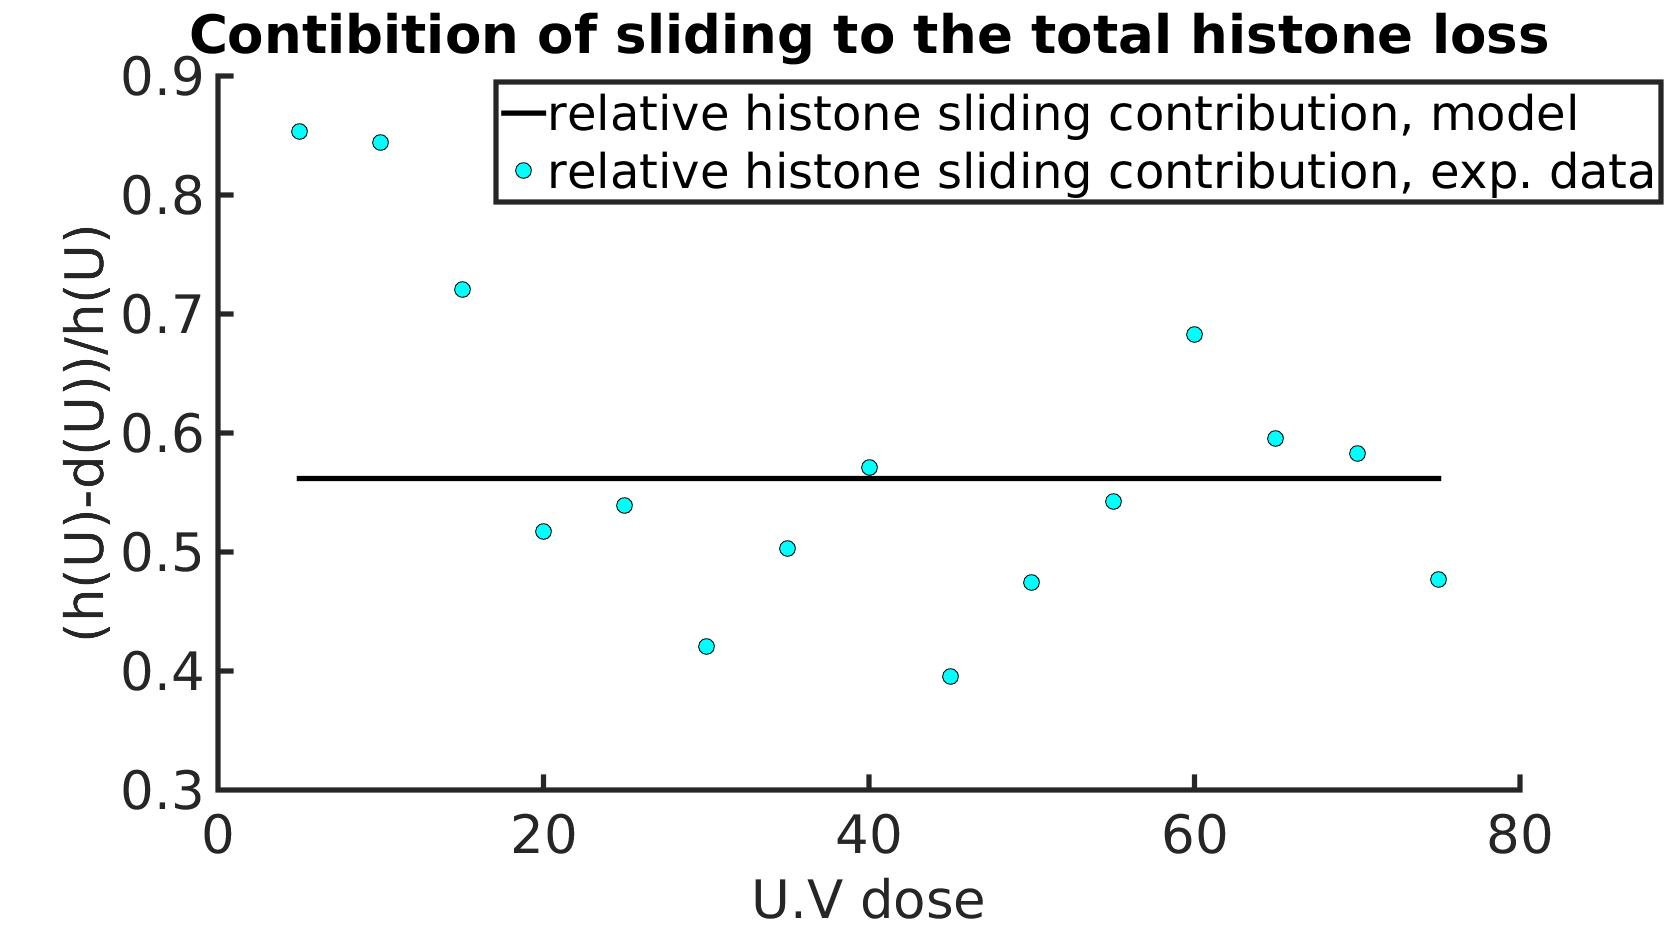
\includegraphics[width=0.5\linewidth, height=0.3\textheight]{relativeSlidingContribution}
\caption{\textbf{Relative contribution of sliding to the total histone loss $(h(U)-d(U))/h(U)$}. It is constant according to our model (black line).}
\label{fig:relativeSlidingContribution}
\end{figure}
%%%%%%%%%%%%%%%%%%%%%%%%%%%%%%%%%%%%%%%%%%%%%%%%%%%%%%%%%%%

%%%%%%%%%%%%%%%%%%%%%%%%%%%%%%%%%%%%%%%%%%%%%%%%%%%%%%%%%%%
\subsection{Relative contribution of sliding and chromatin opening to the expansion of the DR}\label{subsection:RelativecontibutionOfSlidingAndOpeningToExpansion}
%%%%%%%%%%%%%%%%%%%%%%%%%%%%%%%%%%%%%%%%%%%%%%%%%%%%%%%%%%%
The fraction of expansion attributed to both histone sliding and chromatin opening can be computed using eq. \ref{eq:histoneLoss} for the time dependent function of histone loss, and search for the time $\hat{t}=\kappa t_s$, with $0\leq \kappa\leq 1$, for which the histone loss fraction reaches $0.56$, the constant value estimated for $(h(U)-d(U))/h(U)$ (Fig. \ref{fig:relativeSlidingContribution}). Using expressions \ref{eq:histoneLoss} and \ref{eq:totalHistoneLoss}, we solve for $\kappa$ the equation
\begin{equation*}
0.56h(t_s)=1-\frac{\exp(-\kappa C_1)}{ 1+C_2(1-\exp(-\kappa C_1))}
\end{equation*}
to obtain
\begin{equation} \label{eq:timeFractionForHistoneLoss}
\kappa = -\frac{1}{\beta U}\ln{\left( \frac{(1+C_2)(1-0.56h(t_s))}{1+C_2 -0.56C_2h(t_s)}\right)}
\end{equation}
Using $\kappa$ we calculate the relative expansion attributed to sliding by the relation
\begin{equation} \label{eq:relativeSlidingExpansion}
\frac{\alpha(\hat{t})-1}{\alpha (t_s)-1}
\end{equation}
The complementary function $\left(\alpha(t_s)-\alpha(\hat{t})\right) /\left(\alpha(t_s)-1\right)$, is the contribution of chromatin opening to the total expansion of the DR. Plugging \ref{eq:timeFractionForHistoneLoss} into \ref{eq:relativeSlidingExpansion}, we obtain the curve in Figure \ref{fig:histoneAndDNARelativeExpansionContribution}. As can be appreciated from Figure \ref{fig:histoneAndDNARelativeExpansionContribution}, histone sliding and chromatin opening contribute roughly equally to the expansion of the DR, with slight decrease of sliding contribution with increase in UV dose.
The time dependent histone loss behaves in a near linear manner independent of UV dose (data not shown), which allows us to approximate the relative expansion related to histone sliding regardless of the exact time point, but as a function of the total time it takes to lose 56\% of the histones from the ROI. 

We interpret the decreasing relative contribution of histone sliding (Figure \ref{fig:histoneAndDNARelativeExpansionContribution}) to the expansion as the increase in the need for DNA reorganization with increase in UV dose. With increasing UV dose more DNA is damaged in the IDR, which results in more chromatin opening and eventual loss of DNA and histones from the ROI. We note that the mechanism of DNA and histone loss due to chromatin opening contributes to the expansion during histone sliding. However, DNA and histone loss attributed solely to chromatin opening can operate with no sliding. 


\begin{figure}[H]
\centering
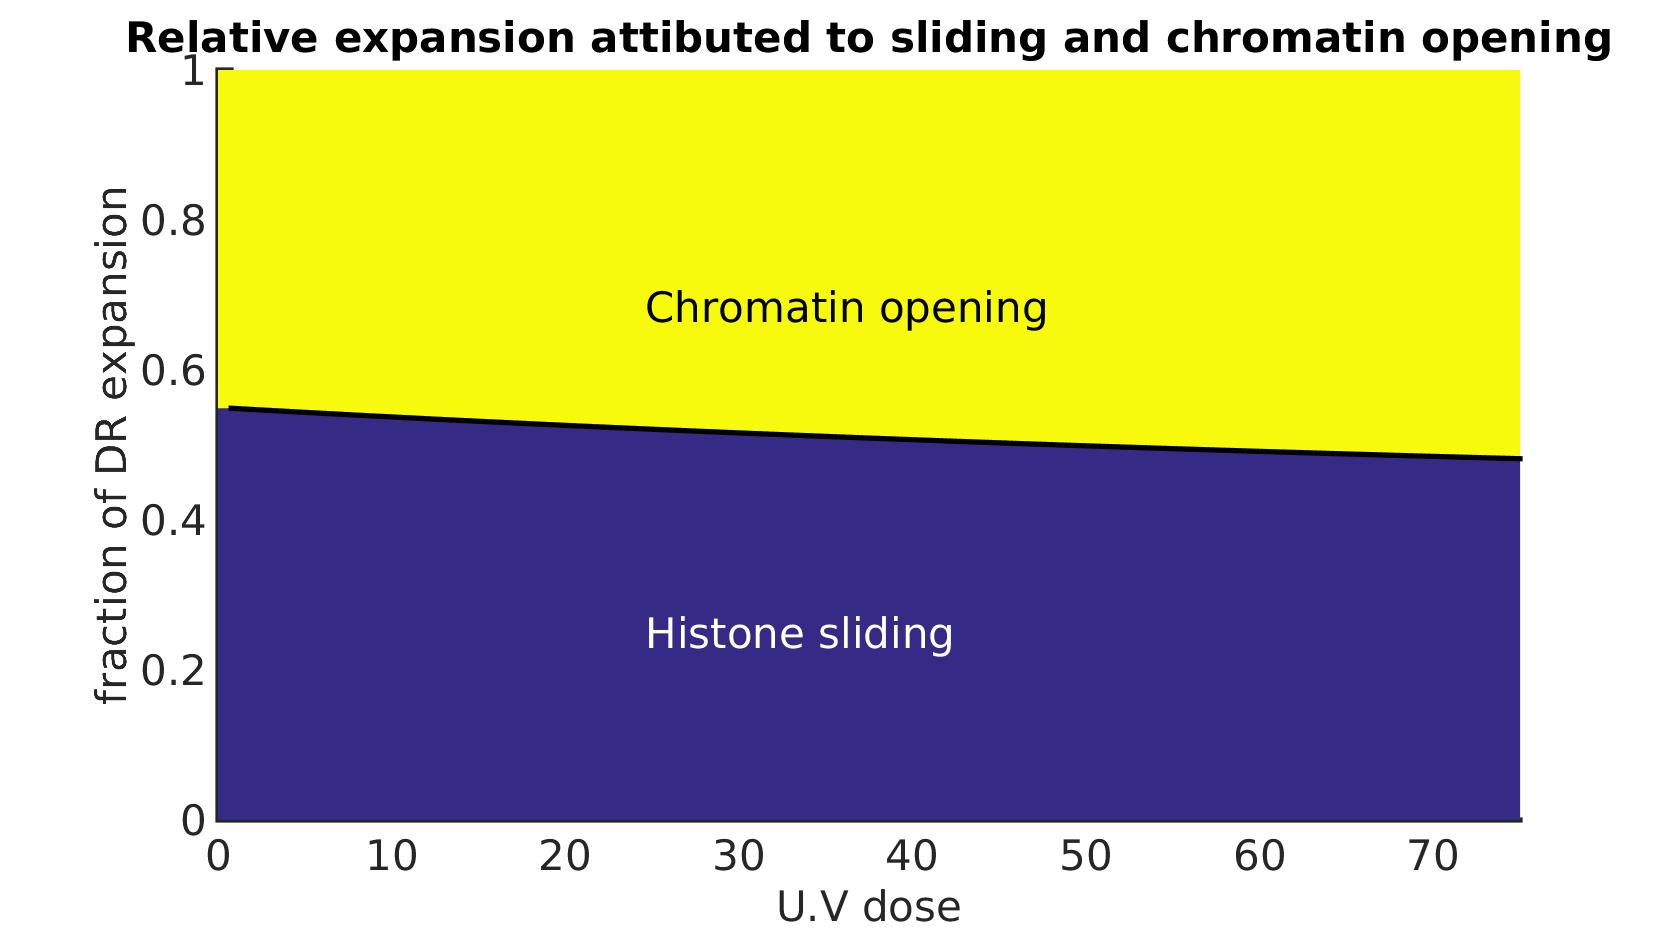
\includegraphics[width=0.5\linewidth, height=0.3\textheight]{histoneAndDNARelativeExpansionContribution}
\caption{\textbf{Relative contribution of histone sliding (purple) and chromatin opening (yellow) to the total expansion of the DR. Roughly 56\% of the total histone loss is attributed to sliding, independent of the UV dose (Figure \ref{fig:relativeSlidingContribution}), for which the relative contribution for the expansion of the DR is slightly decreasing with UV dose. We note that during histone sliding chromatin opening continues to operate, but no conversely.}}
\label{fig:histoneAndDNARelativeExpansionContribution}
\end{figure}


\end{document}

